Official statistics published by the U.S. government~\cite{EducationPaysBureau} indicate that individuals with doctoral degrees belong to a distinguished group characterized by the highest median weekly earnings and the lowest unemployment rates across the country. With the privilege comes responsibility. In recognizing the advantages my educational status affords me, I am committed to leveraging this privilege to foster inclusive excellence in STEM education, where diversity metrics have yet to reach an acceptable standard.

Having attended training programs centered on diversity, equity, and inclusivity (DEI) in STEM education, I have gained a solid understanding that \emph{diversity} in academia extends beyond common identity indicators like race, class, ethnicity, citizenship, gender \& gender identity, sexual orientation, religion, ability, marital status, veteran status, political affiliation, etc. It also includes educational backgrounds and life experiences such as those of transfer students, non-traditional students (e.g., aged 25 and above or those returning to education), student parents, first-generation students, academically under-prepared students, international students, and so on. Capturing the full spectrum of diversity is essential to crafting a truly inclusive educational environment.

The commitment to diversity became even more personal and tangible during a routine COVID test on campus. The young man conducting the test was unaware of what a ``postdoc'' was, revealing a gap in his knowledge of educational pathways, especially regarding doctoral programs. This interaction keeps on reminding me of the broader role that an educator can play. As a future faculty member, I am inspired to be a force of enlightenment and change, to open up opportunities to students who may have never known of the intellectual and life options that abound at our university. The influence of these seemingly simple acts of sharing knowledge and opening doors can be more significant than most people perceive.

\begin{figure}[!ht]
    \centering
    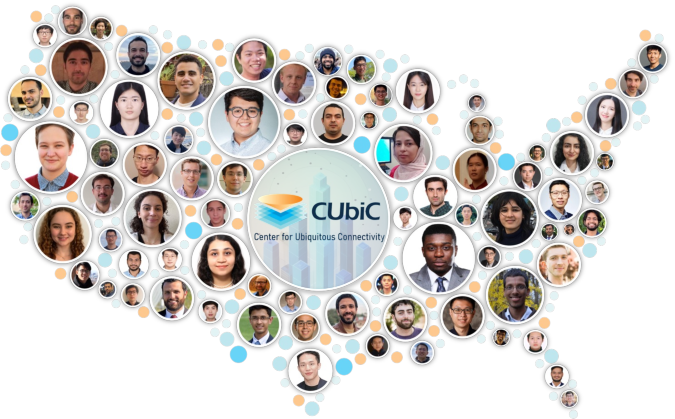
\includegraphics[width=0.5\linewidth]{../../fig/diversity.png}
    \caption{Firsthand experience of diversity in action at the SRC JUMP 2.0 Center for Ubiquitous Connectivity (CUbiC) have profoundly shaped my understanding of inclusive practices in STEM education.}
    \label{fig:diversity}
\end{figure}

My time at the Center for Ubiquitous Connectivity (CUbiC) under the SRC JUMP 2.0 program has been instrumental in shaping my understanding of practical diversity in action. Diversity is a critical priority in the CUbiC center, as evidenced by the center featuring a female director, a female theme lead, 6 female principal investigators, alongside over 20\% and growing researchers from underrepresented groups. Witnessing the center's inclusive mentoring and outreach programs has demonstrated to me the utmost importance of such initiatives in a research environment. These experiences have provided me with a solid framework for what I aspire to emulate in establishing my own research group in the \appDept{} at the \appSchool{}.

In conclusion, it is through the combined efforts\textemdash recognizing the full spectrum of diversity, actively contributing to an inclusive academic culture, and taking every opportunity to educate and inform\textemdash that I aim to fulfill the responsibility that accompanies my privileged educational achievement. I see it as my duty to ensure that the pathways to academic and professional success are accessible to all, and to serve as a mentor for the next generation of scholars and innovators.

